\section{Data Exploration}

\subsection{Dataset overview}

MovieLens 1M contains three core tables:
\begin{itemize}
  \item \textbf{Ratings} (\texttt{userId}, \texttt{movieId}, \texttt{rating}, \texttt{timestamp})
  \item \textbf{Movies} (\texttt{movieId}, \texttt{title}, \texttt{genres})
  \item \textbf{Users} (\texttt{userId}, \texttt{gender}, \texttt{age}, \texttt{occupation}, \texttt{zipCode})
\end{itemize}

The loaded corpus contains \textbf{1{,}000{,}209} ratings from \textbf{6{,}040} users on \textbf{3{,}883} catalog movies
(3{,}706 movies with at least one rating in the interaction matrix).
Matrix sparsity is \textbf{95.74\%}---only about 4.3\% of possible user--movie pairs are observed---which is
typical for explicit-feedback recommenders.

\subsection{Rating distribution}

Users skew toward positive ratings: mean rating \textbf{3.58} stars, median \textbf{4} stars, with the highest
count at 4 stars (Figure~\ref{fig:rating-dist}).
This generosity bias implies that RMSE penalizes under-prediction of high ratings differently than
symmetric error would suggest, and that a global-mean baseline is a meaningful floor.

\begin{figure}[ht]
  \centering
  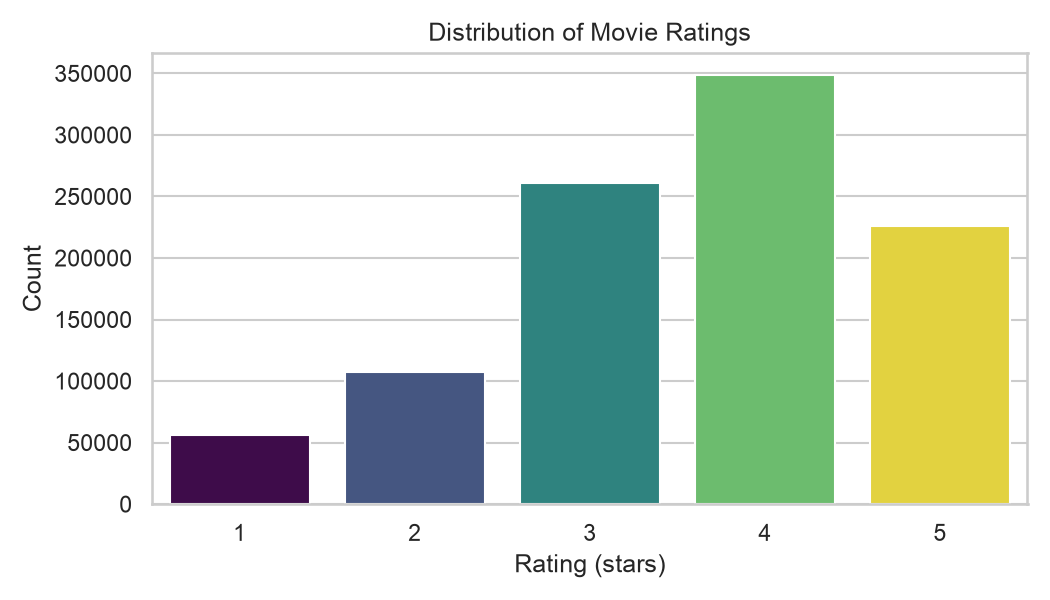
\includegraphics[width=0.75\textwidth]{figures/rating_distribution.png}
  \caption{Distribution of explicit star ratings in MovieLens 1M.}
  \label{fig:rating-dist}
\end{figure}

\subsection{Demographics}

Gender and binned age categories are unevenly distributed (Figure~\ref{fig:demographics}).
Occupation and age codes are categorical; they are included as numeric features in our ML pipeline
for simplicity, though one-hot encoding could be explored in future work.

\begin{figure}[ht]
  \centering
  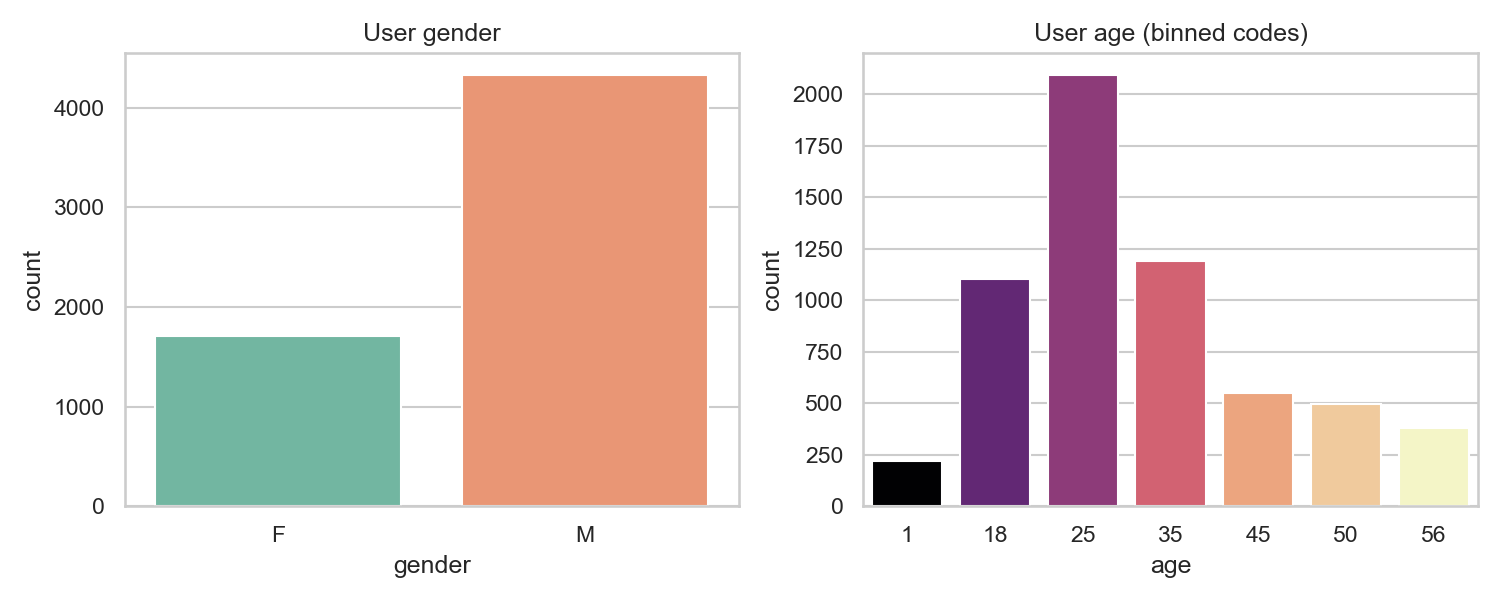
\includegraphics[width=\textwidth]{figures/user_demographics.png}
  \caption{User gender and age-bin distributions.}
  \label{fig:demographics}
\end{figure}

\subsection{Long tail and cold start}

Movie popularity is highly skewed: a small head of blockbusters accumulates thousands of ratings,
while \textbf{663} movies (17.9\% of rated titles) receive fewer than 20 ratings---our cold-start threshold
(Figure~\ref{fig:long-tail}).
User activity is similarly skewed: \textbf{1{,}743} users (28.9\%) submitted fewer than 50 ratings
(Figure~\ref{fig:user-activity}).

\begin{figure}[ht]
  \centering
  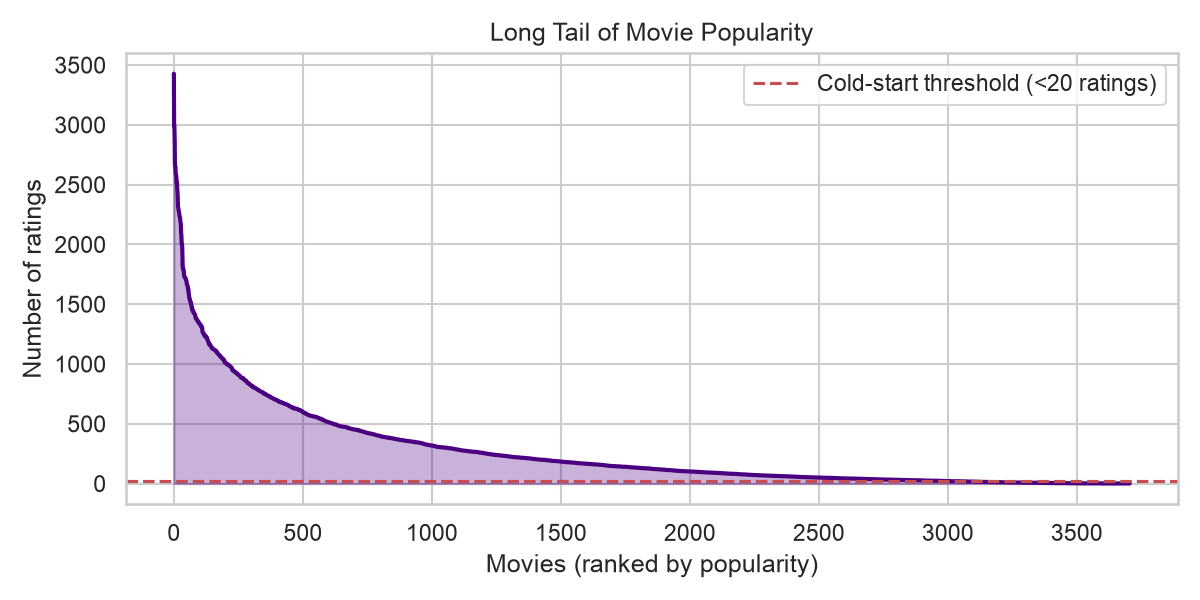
\includegraphics[width=0.85\textwidth]{figures/long_tail.png}
  \caption{Long-tail distribution of movie popularity (ranked by rating count).}
  \label{fig:long-tail}
\end{figure}

\begin{figure}[ht]
  \centering
  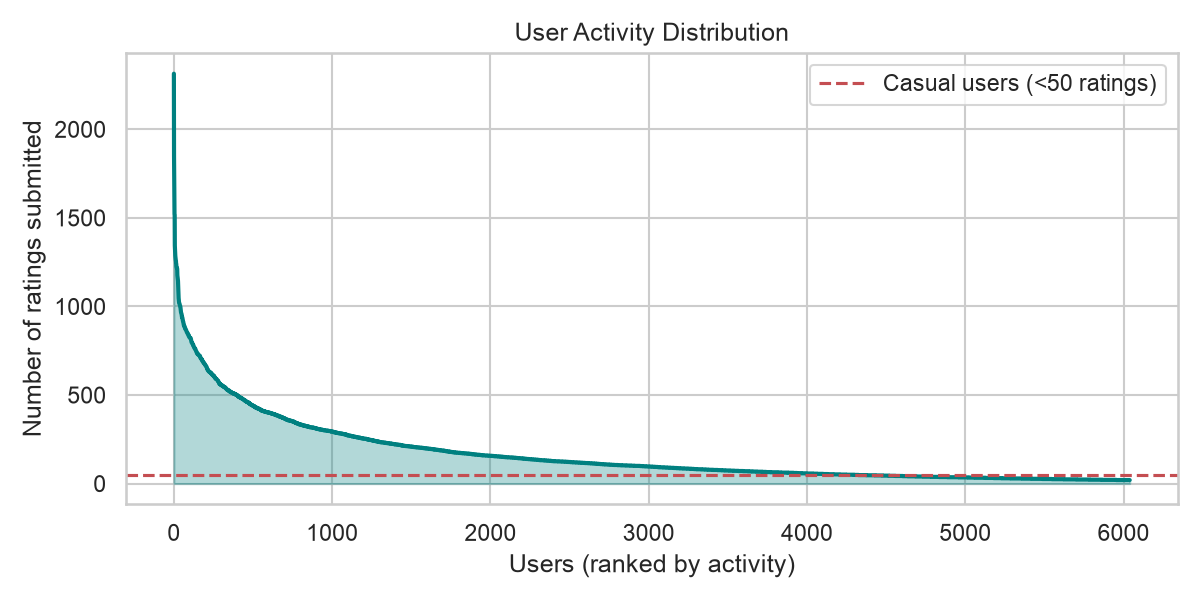
\includegraphics[width=0.85\textwidth]{figures/user_activity.png}
  \caption{Distribution of user rating activity.}
  \label{fig:user-activity}
\end{figure}

These patterns motivate:
\begin{itemize}
  \item Popularity and average-rating features at the movie level.
  \item Activity and average-rating features at the user level.
  \item Hybrid models that do not rely solely on pairwise co-occurrence for tail items.
\end{itemize}

The same plots are reproduced in \texttt{notebooks/MovieMind\_capstone.ipynb} (Section~2).
Regenerate figures with: \texttt{python3 docs/report/generate\_figures.py} from the project root.
